\documentclass[a4paper]{article}
\synctex=1
\usepackage[T1]{fontenc}
\usepackage{tikz,graphicx,siunitx,amssymb,amsmath,a4wide}
\usepackage[backend=biber]{biblatex}

\usetikzlibrary{plotmarks,arrows}

\newcommand{\vSI}[2]{\SI[math-rm=\ensuremath,parse-numbers=false]{#1}{#2}}


\title{
  UPC Manresa Ventilator Unit\\
  Control Software}
\author{
  Sebas Vila\\
  Manresa School of Engineering\\
  Universitat Politècnica de Catalunya}

\addbibresource{local.bib}


\begin{document}
\maketitle{}


\section{Introduction}
\label{sec:introduction}

The COVID19 pandemia crisis raised the need to make available
mechanical ventilation units to assist patients during the critical
phases of the dissease. Several initiatives around the world appeared
with this objective,\cite{}. The «UPC Ventilation Unit», in what
follows UPC-VU, was an initiative held at UPC's Manresa School of
Engineering that targets the design of a reliable low cost and easy to
build ventilation unit. UPC-VU follows the roughly idea of designing
an electromechanical system that runs through an Ambu like manual
resuscitation device, \cite{a.s.20:_ambu_oval_silic_resus}. This makes
easy to use standart piping and to avoid contamination related issues.

\begin{figure}[tb]
  \centering
  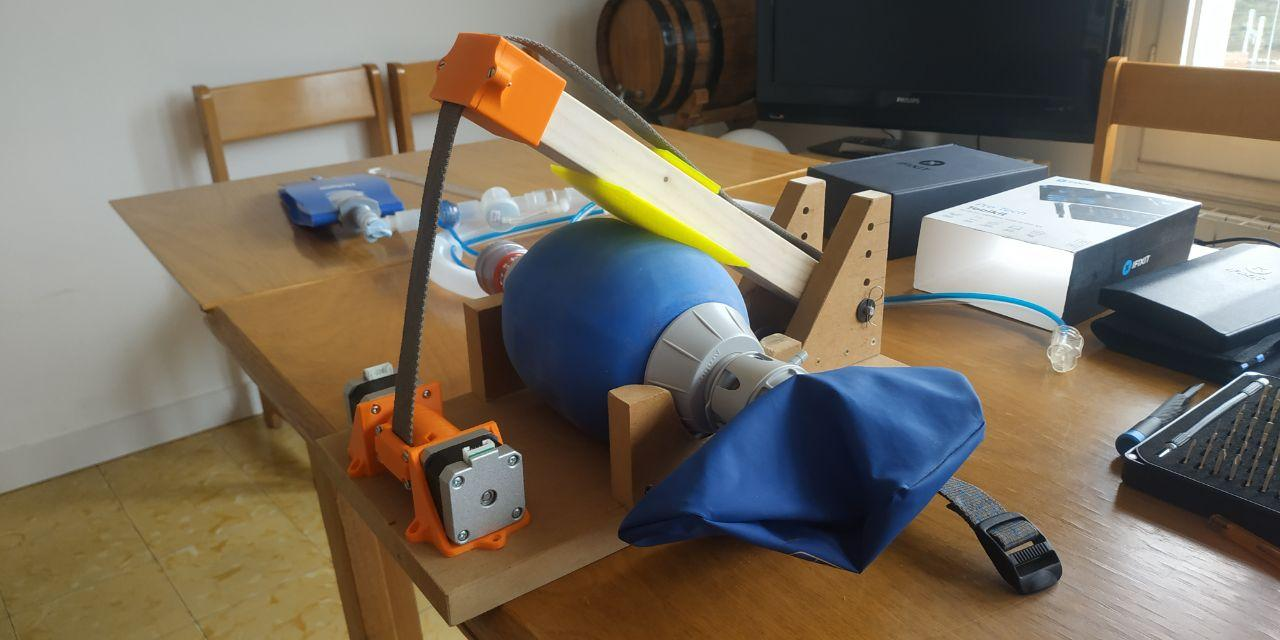
\includegraphics[width=0.7\textwidth]{upc-vu-v1}
  \label{fig:upc-vu}
  \caption{A prototype of UPC Ventilation Unit}
\end{figure}

The UPC-VU, see Fig~\ref{fig:upc-vu}, power is given by an standard
NEMA~XX 200 poles stepper motor. In this context is of capital
importance to give the motor the precise motion to achieve the desired
inpiration/expiration behaviour. This manuscript develops an algorithm
to move the motor following a suitable profile.
% why???
We focused on the inspiration motion.

% explain some ideas about the mechanical part to better introduce the report

After this introduction, the manuscript is organized as follows.




\section{Ventilator cycle model}
\label{sec:vent-cycle-model}

In this section we explain the VU motion profile. This profile defines
the dynamic rotation of the motor with respect to the time. We assume
that the motor rotation profile is correlated to the flux and volume of
insufflated air.

The VU follows a periodic profile. The
figure~\ref{fig:ventilation-profile} shows a single period of the
profile. The main characteristics of the profile are defined by a set
of parameters. The end user modifies the parameters to dynamically
change the profile. While most of the parameters can be interactively
tunned by the end user, a small part remain constant and they are
considered system constants.

Time notation is sometimes confusing. In what follows we will
distinguish between time durations and time instants. Time instants
will always be referred to $t_0$, the beginning of a breathe
cycle. This manuscript will use plain names to denote time durations
as $\mathit{ir}$ and $t_{\mathit{ir}}$ to denote time instants, see
figure~\ref{fig:ventilation-profile}.

The set of parameters is the following.

\begin{figure}[tb]
  \centering
  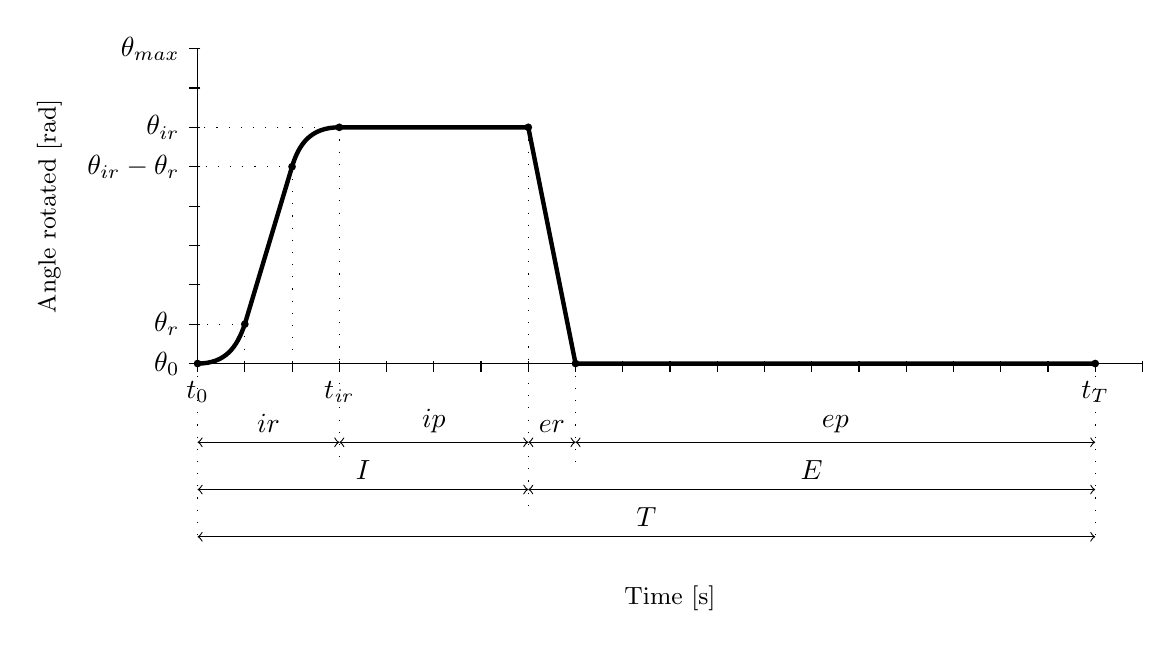
\begin{tikzpicture}[y=0.5cm, x=0.6cm]
    % axis
    \draw (0,0) -- coordinate (x axis mid) (20,0);
    \draw (0,0) -- coordinate (y axis mid) (0,8);
    % ticks
    \foreach \x in {0,...,20}
    \draw (\x,1pt) -- (\x,-3pt);
    \foreach \y in {0,...,8}
    \draw (1pt,\y) -- (-3pt,\y);
    % axis labels      
    \node[below=2.7cm] at (x axis mid)
    {\small Time [s]};
    \node[rotate=90, above=1.6cm] at (y axis mid)
    {\small Angle rotated [rad]};
    % main coordinates
    \coordinate (beg-insp)     at (0,0) ;
    \coordinate (end-insp-acc) at (1,1) ;
    \coordinate (end-insp-lin) at (2,5) ;
    \coordinate (end-insp-dec) at (3,6) ;
    \coordinate (end-insp-pau) at (7,6) ;
    \coordinate (end-exp)      at (8,0) ;
    \coordinate (end-exp-pau)  at (19,0);
    % draw angle function
    \draw [ultra thick] plot
    (beg-insp) .. controls +(0:0.6) and +(254:0.6) ..
    (end-insp-acc) --
    (end-insp-lin) .. controls +(76:0.6) and +(180:0.6) ..
    (end-insp-dec) --
    (end-insp-pau) --
    (end-exp) --
    (end-exp-pau);
    % draw special dots on curve
    \fill (beg-insp)     circle(1.4pt);
    \fill (end-insp-acc) circle(1.4pt);
    \fill (end-insp-lin) circle(1.4pt);
    \fill (end-insp-dec) circle(1.4pt);
    \fill (end-insp-pau) circle(1.4pt);
    \fill (end-exp)      circle(1.4pt);
    \fill (end-exp-pau)  circle(1.4pt);
    % draw vertical reference lines
    \draw [thin,loosely dotted] plot (end-insp-acc) -- (end-insp-acc|-0,0);
    \draw [thin,loosely dotted] plot (end-insp-lin) -- (end-insp-lin|-0,0);
    \draw [thin,loosely dotted] plot (end-insp-dec) -- (end-insp-dec|-0,0);
    \draw [thin,loosely dotted] plot (end-insp-pau) -- (end-insp-pau|-0,0);
    % draw horizontal reference lines
    \draw [thin,loosely dotted] plot (end-insp-acc) -- (end-insp-acc-|0,0);
    \draw [thin,loosely dotted] plot (end-insp-lin) -- (end-insp-lin-|0,0);
    \draw [thin,loosely dotted] plot (end-insp-dec) -- (end-insp-dec-|0,0);
    % x axis annotations
    \draw (0,-3pt) node[anchor=north] {$t_0$};
    \draw (end-insp-dec |- 0,-3pt) node[anchor=north] {$t_\mathit{ir}$};
    \draw (end-exp-pau |- 0,-3pt) node[anchor=north] {$t_T$};
    % y axis annotations
    \draw (-3pt,0) node[anchor=east] {$\theta_0$};
    \draw (end-insp-acc-|-3pt,0) node[anchor=east] {$\theta_{r}$};
    \draw (end-insp-lin-|-3pt,0) node[anchor=east] {$\theta_{ir}-\theta_r$};
    \draw (end-insp-dec-|-3pt,0) node[anchor=east] {$\theta_{ir}$};
    \draw (-3pt,8) node[anchor=east] {$\theta_{max}$};
    % draw important time intervals
    \draw [thin]
    (beg-insp|-0,-4.4) edge[<->] node[above] {$T$} (end-exp-pau|- 0,-4.4);
    \draw [thin]
    (beg-insp|-0,-3.2) edge[<->] node[above] {$I$} (end-insp-pau|- 0,-3.2);
    \draw [thin]
    (end-insp-pau|-0,-3.2) edge[<->] node[above] {$E$} (end-exp-pau |- 0,-3.2);
    \draw [thin]
    (beg-insp|-0,-2) edge[<->] node[above] {$ir$} (end-insp-dec |- 0,-2);
    \draw [thin]
    (end-insp-pau|-0,-2) edge[<->] node[above] {$er$} (end-exp |- 0,-2);
    \draw [thin]
    (end-insp-dec|-0,-2) edge[<->] node[above] {$ip$} (end-insp-pau |- 0,-2);
    \draw [thin]
    (end-exp|-0,-2) edge[<->] node[above] {$ep$} (end-exp-pau |- 0,-2);
    % draw time intervals reference lines
    \draw [thin,loosely dotted] plot (beg-insp)     -- (beg-insp    |-0,-4.6);
    \draw [thin,loosely dotted] plot (end-insp-dec) -- (end-insp-dec|-0,-2.5);
    \draw [thin,loosely dotted] plot (end-insp-pau) -- (end-insp-pau|-0,-3.7);
    \draw [thin,loosely dotted] plot (end-exp)      -- (end-exp     |-0,-2.5);
    \draw [thin,loosely dotted] plot (end-exp-pau)  -- (end-exp-pau |-0,-4.6);
  \end{tikzpicture}
  \label{fig:ventilation-profile}
  \caption{Ventilation cycle profile.}
\end{figure}

\begin{description}
  
\item[breathing rate] The breathing rate, $\mathit{rr}$, defines the
  breathing frequency. Usually measured in breathing cycles per
  minute. The period $T$ in [\si{\second}] can be obtained as:
  $$
  \boxed{
    T = \bigg(\frac{60}{\mathit{rr}}\bigg)^{-1} = \frac{\mathit{rr}}{60}
  }
  $$
  This parameter can be tunned by the end user.

\item[I:E ratio] The breathing cycle is the concatenation of two
  phases known as inspiration and expiration. In
  figure~\ref{fig:ventilation-profile}, the inspiration time is
  labeled as $I$ while the expiration time is labeled as $E$. The
  ratio between both times, $I:E$, is usually shown by normalizing $I$
  to $1$. Thus, currently we use ratios like $1:2$ or $1:1.3$. Given a
  ratio $1:k$, we name $k$ as the ``I:E ratio''. Let $I$ be the
  inspiration time and let $E$ be the expiration time, then,
  $$
  k=\frac{E}{I}
  $$
  This parameter can be tunned by the end user.
  
\item[inspiration ramp time] The time spent compressing the Ambu is
  named ``inspiration ramp time'' and noted as $\mathit{ir}$.
  This parameter can be tunned by the end user.
  
\item[travel] The UPC ventilator unit mechanism works by winding a
  rope to a motor shaft. This induces a compression on the Ambu using
  a lever. The maximum angle that the motor shaft can turn to obtain
  the greatest compression is noted as $\theta_\textit{max}$. By
  turning an angle $\theta<\theta_\textit{max}$ we obtain a smaller
  air volume. The ``travel'', noted as $\mathit{tr}$, is the actual
  percentage of angle turned with respect to the maximum. Then, the
  actual angle turned $\theta_{ir}$ is
  $$
  \boxed{
    \theta_{ir} = \frac{\mathit{tr}\cdot\theta_\mathit{max}}{100}
  }
  $$
  This parameter can be tunned by the end user.
  
\item[expiration ramp time] The expiration ramp time, noted as
  $\mathit{er}$. This parameter is considered a constant parameter
  that cannot be tunned by the end user.

\end{description}


The parameters explained before fully define the time characteristics
of the ventilation cycle. However, as shown in the
figure~\ref{fig:ventilation-profile}, there are additional variables
which are interesting. In what follows we obtain the values of $E$,
$I$, $\mathit{ip}$ and $\mathit{ep}$ from the system parameters.

Assume that $T$ and $k$, the I:E ratio, are known parameters. Then,
times $E$ and $I$ can be computed following this equation
\begin{equation*}
  \left.
    \begin{aligned}
      I+E &= T \\
      kI  &= E \\
    \end{aligned}
  \right\}
\end{equation*}
which leads to
\begin{equation}
  \label{eq:19}
  \boxed{
    I = \frac{T}{k+1} \qquad E = \frac{kT}{k+1}
  }
\end{equation}

In the figure~\ref{fig:ventilation-profile}, $\mathit{ip}$ and
$\mathit{ep}$ are the duration of the inspiration and expiration
pauses, respectively. Assume that $T$, $\mathit{ir}$, $\mathit{er}$
and the ratio $k$ are known parameters. Then, $\mathit{ip}$ and
$\mathit{ep}$ can be obtained by the equation
\begin{equation*}
  \left.
    \begin{aligned}
      \mathit{ir}+\mathit{ip}+\mathit{er}+\mathit{ep} &= T \\
      k(\mathit{ir}+\mathit{ip}) &= \mathit{er}+\mathit{ep}
    \end{aligned}
  \right\}
\end{equation*}
by replacing the second equation on the first we obtain
\begin{equation*}
  \begin{split}
    T &= \mathit{ir}+\mathit{ip}+k(\mathit{ir}+\mathit{ip}) \\
      &= (k+1)\mathit{ir} + (k+1)\mathit{ip}
  \end{split}
\end{equation*}
which results in
\begin{equation}
  \label{eq:20}
  \boxed{
    \mathit{ip} = \frac{T-(k+1)\mathit{ir}}{k+1}
  }
\end{equation}
applying the last result to the first equation conduces to
\begin{equation*}
  T = \mathit{ir}+\frac{T-(k+1)\mathit{ir}}{k+1}+\mathit{er}+\mathit{ep}\\
\end{equation*}
from where
\begin{equation*}
  \begin{split}
    \mathit{ep} &=
    T-\mathit{ir}-\mathit{er}-\frac{T-(k+1)\mathit{ir}}{k+1}\\
    &=
    \frac{(k+1)T-(k+1)\mathit{ir}-(k+1)\mathit{er}-T+(k+1)\mathit{ir}}
    {k+1}\\
    &= \frac{kT-(k+1)\mathit{er}}{k+1}
  \end{split}
\end{equation*}
then
\begin{equation}
  \label{eq:25}
  \boxed{
    \mathit{ep} = \frac{kT-(k+1)\mathit{er}}{k+1}
  }
\end{equation}


\subsection{Inspiration ramp shape}

\begin{figure}[tb]
  \centering
  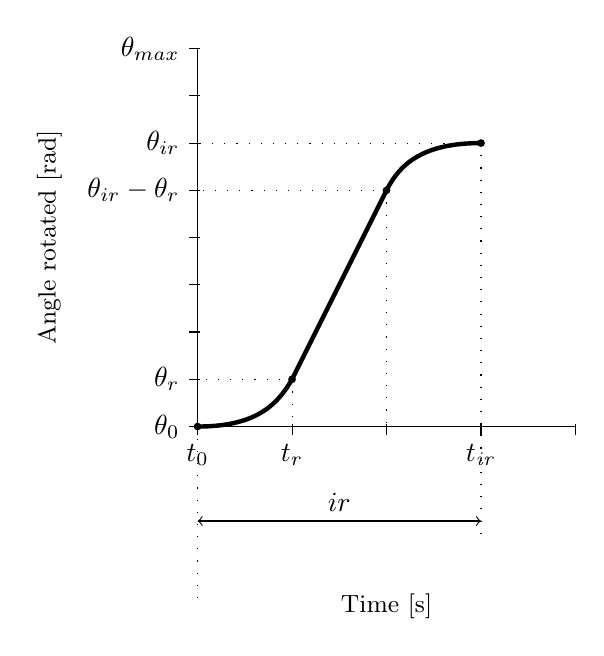
\begin{tikzpicture}[y=0.6cm, x=1.2cm]
    % axis
    \draw (0,0) -- coordinate (x axis mid) (4,0);
    \draw (0,0) -- coordinate (y axis mid) (0,8);
    % ticks
    \foreach \x in {0,...,4}
    \draw (\x,1pt) -- (\x,-3pt);
    \foreach \y in {0,...,8}
    \draw (1pt,\y) -- (-3pt,\y);
    % axis labels      
    \node[below=2cm] at (x axis mid)
    {\small Time [s]};
    \node[rotate=90, above=1.6cm] at (y axis mid)
    {\small Angle rotated [rad]};
    % main coordinates
    \coordinate (beg-insp)     at (0,0) ;
    \coordinate (end-insp-acc) at (1,1) ;
    \coordinate (end-insp-lin) at (2,5) ;
    \coordinate (end-insp-dec) at (3,6) ;
    % draw angle function
    \draw [ultra thick] plot
    (beg-insp) .. controls +(0:0.6) and +(254:0.6) ..
    (end-insp-acc) --
    (end-insp-lin) .. controls +(76:0.6) and +(180:0.6) ..
    (end-insp-dec);
    % draw special dots on curve
    \fill (beg-insp)     circle(1.4pt);
    \fill (end-insp-acc) circle(1.4pt);
    \fill (end-insp-lin) circle(1.4pt);
    \fill (end-insp-dec) circle(1.4pt);
    % draw vertical reference lines
    \draw [thin,loosely dotted] plot (end-insp-acc) -- (end-insp-acc|-0,0);
    \draw [thin,loosely dotted] plot (end-insp-lin) -- (end-insp-lin|-0,0);
    \draw [thin,loosely dotted] plot (end-insp-dec) -- (end-insp-dec|-0,0);
    % draw horizontal reference lines
    \draw [thin,loosely dotted] plot (end-insp-acc) -- (end-insp-acc-|0,0);
    \draw [thin,loosely dotted] plot (end-insp-lin) -- (end-insp-lin-|0,0);
    \draw [thin,loosely dotted] plot (end-insp-dec) -- (end-insp-dec-|0,0);
    % x axis annotations
    \draw (0,-3pt) node[anchor=north] {$t_0$};
    \draw (end-insp-acc |- 0,-3pt) node[anchor=north] {$t_r$};
    \draw (end-insp-dec |- 0,-3pt) node[anchor=north] {$t_\mathit{ir}$};
    % y axis annotations
    \draw (-3pt,0) node[anchor=east] {$\theta_0$};
    \draw (end-insp-acc-|-3pt,0) node[anchor=east] {$\theta_{r}$};
    \draw (end-insp-lin-|-3pt,0) node[anchor=east] {$\theta_{ir}-\theta_r$};
    \draw (end-insp-dec-|-3pt,0) node[anchor=east] {$\theta_{ir}$};
    \draw (-3pt,8) node[anchor=east] {$\theta_{max}$};
    % draw important time intervals
    \draw [thin]
    (beg-insp|-0,-2) edge[<->] node[above] {$ir$} (end-insp-dec |- 0,-2);
    % draw time intervals reference lines
    \draw [thin,loosely dotted] plot (beg-insp)     -- (beg-insp    |-0,-3.7);
    \draw [thin,loosely dotted] plot (end-insp-dec) -- (end-insp-dec|-0,-2.5);
  \end{tikzpicture}
  \label{fig:S-shape-profile}
  \caption{Ventilation ramp S-shape profile.}
\end{figure}

The inspiration ramp has an S-shape profile that smoothes the motor
motion. The figure~\ref{fig:S-shape-profile} focuses on this ramp. The
ramp exhibits three main sections: (i) a constant acceleration
section; (ii) a constant speed section; and (iii) a constant
deceleration section. The acceleration and the deceleration sections
are symmetrical.

The speedup section ratio, $\mathit{ssr}\in(0,0.5]$, is the system
parameter which defines the inspiration ramp shape. It cannot be
tunned by the end user.
%
Specifically, $\mathit{ssr}$ defines the size of the acceleration and
deceleration sections.

Let $\theta_{ir}$ be the angular travel of the actual profile. Then,
given $\mathit{ssr}$, the S-shape profile is defined as follows. The
acceleration section spans from $\theta_0$ to
$\theta_r=\mathit{ssr}\cdot\theta_{ir}$; the constant speed section
goes from $\theta_r$ to $\theta_{ir}-\theta_r$; and the deceleration
section spans from $\theta_{ir}-\theta_r$ to $\theta_{ir}$. Note that
the sections are defined over the turned angle.

The figure~\ref{fig:profile}, shows a complementary view of the
inspiration ramp S-shaped profile. This view shows the angular speed
in function of the turned angle. Note that in central section
rotational speed $\omega_r$ is constant while in the first and the
last sections there is a constant acceleration $\omega'_r$ and
deceleration $-\omega'_r$, respectively.

Given this profile of speeds we are faced to a new problem. We need to
determine which are the values of $\omega_r$ and $\omega_r'$ that
should be applied to inspiration ramp. The next subsection is devoted
to solve this issue.

\begin{figure}[tb]
  \centering
  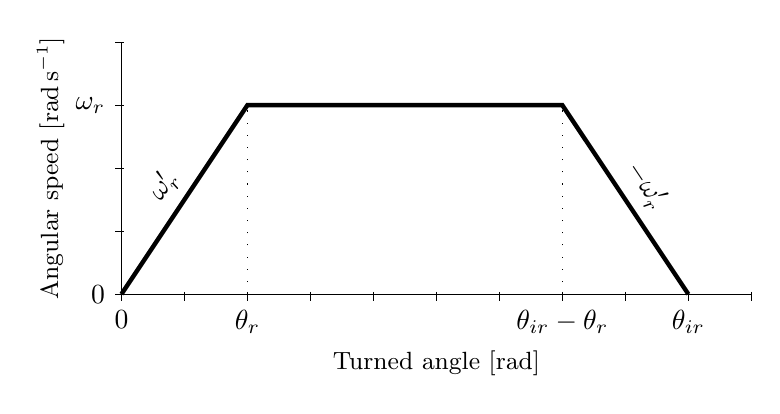
\begin{tikzpicture}[y=.2cm, x=1cm,scale=0.8]
    % axis
    \draw (0,0) -- coordinate (x axis mid) (10,0);
    \draw (0,0) -- coordinate (y axis mid) (0,20);
    % ticks
    \foreach \x in {0,...,10}
    \draw (\x,1pt) -- (\x,-3pt);
    \foreach \y in {0,5,...,20}
    \draw (1pt,\y) -- (-3pt,\y);

    % 
    \draw (0,-3pt) node[anchor=north] {$0$};
    \draw (2,-3pt) node[anchor=north] {$\theta_r$};
    \draw (7,-3pt) node[anchor=north] {$\theta_{ir}-\theta_r$};
    \draw (9,-3pt) node[anchor=north] {$\theta_{ir}$};

    \draw (-3pt,0) node[anchor=east] {$0$};
    \draw (-3pt,15) node[anchor=east] {$\omega_r$};
    
    % axis labels      
    \node[below=0.6cm] at (x axis mid)
    {\small Turned angle [\si{\radian}]};
    \node[rotate=90, above=0.6cm] at (y axis mid)
    {\small Angular speed [\si{\radian\per\second}]};

    % annotated line
    \draw [ultra thick] plot
    (0,0)  -- node[midway,above,sloped]{$\omega_r'$}
    (2,15) --
    (7,15) -- node[midway,above,sloped]{$-\omega_r'$}
    (9,0);
    \draw [thin,loosely dotted] plot (2,0) -- (2,15);
    \draw [thin,loosely dotted] plot (7,0) -- (7,15);
  \end{tikzpicture}
  \label{fig:profile}
  \caption{Inspiration ramp angular speed in function of turned angle.}
\end{figure}


\subsection{Inspiration ramp speed and acceleration values}
\label{sec:comp-prof-param}

The inspiration ramp S-shaped profile is fully defined by three
parameters: the inspiration ramp time $\mathit{ir}$, the total angle
turned $\theta_{ir}$, and the speedup section ratio $\mathit{ssr}$.
%%% NOTA: en aquest apartat T ha de canviar-se per \mathit{ir}

According the previous section, $\mathit{ssr}$ determines the angle
turned during speedup section $\theta_r$. In what follows we will
consider $\theta_r$ instead of $\mathit{ssr}$.

The goal of this section is to work out the values of $\omega_r$ and
$\omega'_r$ given the parameters $\mathit{ir}$, $\theta_{ir}$, and
$\theta_r$.

In what follows, assume that $\theta$, $\omega$ and $\omega'$ will
denote a turned angle, an angular speed and an angular acceleration,
respectively.


% Assume that $\theta_{ir}$ is the total angle turned by the motor
% following the inspiration ramp S-profile, $\theta_r$ is the angle
% turned by the motor at the end of the speedup ramp, and $ir$ the total
% time spent during the profile motion, see
% figure~\ref{fig:ventilation-profile}.

% begin workout

Assume that $t_r$ is the time spent to turn the acceleration section
angle $\theta_r$. Then, the total angle turned at the end of the
acceleration section is given by kinematic basic equation
$\theta_r=\frac{\omega_r' t_r^2}{2}$. Thus,
\begin{equation}
  \label{eq:22}
  t_r = \sqrt{\frac{2\theta_r}{\omega_r'}}
\end{equation}

The angular speed reached at the end of the acceleration section can
be obtained by applying the basic equation $\omega=\omega' t$ and
Eq.~(\ref{eq:22}),
\begin{equation}
  \label{eq:23}
  \boxed{
    \omega_r=\omega_r' t_t= \omega_r' \sqrt{\frac{2\theta_r}{\omega_r'}} = \sqrt{2\theta_r\omega_r'}
  }
\end{equation}
note that $\omega_r$ is the constant angular velocity of the middle
section of the movement.

By applying the fundamental constant speed equation
$t=\frac{\theta}{\omega}$ and the result of Eq.~(\ref{eq:23}), the time
spent in the middle section, say $t_m$, can be obtained as follows
\begin{equation}
  \label{eq:24}
  t_m = \frac{\theta_{ir}-2\theta_r}{\sqrt{2\theta_r\omega_r'}}
\end{equation}

Given the results (\ref{eq:22}) and (\ref{eq:24}) the following
equation on the inspiration ramp total time $\mathit{ir}$ holds:
\begin{eqnarray}
  \label{eq:1}
  ir &=& 2t_r + t_m \\
    &=& 2\sqrt{\frac{2\theta_r}{\omega_r'}} +
        \frac{\theta_{ir}-2\theta_r}{\sqrt{2\theta_r\omega_r'}}
\end{eqnarray}

Because $\mathit{ir}$, $\theta_{ir}$ and $\theta_r$ are known, the value of
$\omega_r'$ can be worked out from the previous equation. By using the
symbolic calculator \texttt{SymPy}, \cite{team20:_sympy}, we got the
following result,
\begin{equation}
  \label{eq:3}
  \boxed{
    \omega_r' = \frac{\theta_{ir}^2 + 4\theta_{ir}\theta_r + 4\theta_r^2}{2\theta_{ir} \mathit{ir}^2}
  }
\end{equation}





\section{Motion profile characteristics}
\label{sec:basic-prof-char}

The motion profile we are interested in a is piecewise linear one as
shown on Fig.~\ref{fig:profile}. The overall motion is of
\vSI{\theta_T}{\radian} The profile is symmetrical and exhibits three
sections.
\begin{enumerate}
\item A speedup ramp that extends during the first $\theta_r$ angular
  displacement.
\item A constant angular speed motion that lasts for $\theta_m$
  angular displacement.
\item A decelerating ramp ---symmetrical to the initial speedup
  ramp--- that lasts for a $\theta_r$ angular displacement.
\end{enumerate}
Thus, the angular motion $\theta_m$ of the middle section accounts for
\begin{equation}
  \label{eq:2}
\theta_m=\theta_T-2\theta_r
\end{equation}


The problem is now how to appropiately drive the stepper motor to get
this kind of profile. Moreover, some parameters of the profile should
be adjustable:
\begin{itemize}
\item The total time spent in the motion, denoted by $T$.
\item The total angular motion induced by the profile, denoted by
  $\theta_T$.
\item The angular motion during the speedup section, denoted by $\theta_r$.
\end{itemize}
In what follows we give a practical but theoretically sound solution
to these issues.


\section{Constant accelerated motion}
\label{sec:const-accel-moti}

In this section we elaborate on a method to generate a seqüence of
steps suitable for giving a stepper motor a constant accelerated
angular motion. This section closely follows the method of Austin,
\cite{austin05:_gener}.

Assume that a stepper motor is driven by sending it a digital pulse
that makes the motor to advance one step. Because this correspondence
between pulses sent to the motor and steps, we will use (motor) pulse ot
(motor) step as equivalent terms. If pulses are sent at regular time
intervals the motor shaft rotates at a constant speed. The actual
speed is related to the time interval used: longuer time intervals
means slower angular speed.
%
To achieve an angular constant accelerated motion the time between
pulses should decrease step to step. The time between pulses should
follow some rule related to the angular acceleration to be obtained.

This section is devoted to the development of an algorithm that
computes the sequence of times between pulses needed to achieve a
given angular acceleration. Moreover, the algoritm designed will be
implementable using the scarce resources of a typical
microcontroler. Additionally, some insights on how to go from an
acceleration to a distinct one will be given.


\subsection{Discrete time}

In what follows we will assume the existence of a base timer that
discretizes the time dimension. Timer will tick at a constant
frequency of \vSI{f}{\hertz}. This means that time between two motor
pulses must be a multiple of the timer period. We will denote by
$c\in\mathbb{N}$ the number of ticks between two consecutive motor
pulses. Then, the time between two motor steps is
\begin{equation}
  \label{eq:4}
  t = \frac{c}{f}  
\end{equation}

\subsection{Constant angular speed}

If we send pulses to the motor every $c$ ticks and assume that $c$ is
a constant value we obtain a constant angular speed
\vSI{\omega}{\radian\per\second} in the motor shaft. This speed is,
\begin{equation}
  \label{eq:5}
  \omega = \frac{\alpha}{\frac{c}{f}} = \frac{\alpha f}{c}  
\end{equation}
being $\alpha$ a characteristic of the motor that describes the angle
rotated in one step. For instance, if a motor has $200$ steps, its
$\alpha$ (\si{\radian}) is
$\alpha = \frac{2\pi}{200} = \frac{\pi}{100}$.


\subsection{Accelerated angular speed}

Let's denote a tick by this symbol: $\uparrow$. Then, consider the
sequence of pulses and tick counts in between:
$\uparrow c_1\uparrow c_2\uparrow\dots$. If $c_1 > c_2$ motor is
accelerating. Aplying fundamental kinematic equation and replacing
Eq.~(\ref{eq:5}) acceleration $\omega'$ is
\begin{equation}
  \label{eq:6}
  \begin{split}
    \omega' & = \frac{\omega_2-\omega_1}{\delta t} \\
            & = \frac{2\alpha f^2(c_1-c_2)}{c_1 c_2 (c_1 + c_2)}
\end{split}
\end{equation}

Consider a rampup with constant acceleration $\omega'$. Then the
angular speed $\omega$ is a function of time: $\omega(t) = \omega'
t$. Integration gives the motor shaft turn angle as a function of
time,
\begin{equation}
  \label{eq:7}
  \theta(t) = \int_0^t \omega(\tau)d\tau = \frac{\omega't^2}{2}  
\end{equation}

Assume that to move $n$ steps the motor shaft we spend a time of
\vSI{t_n}{\second}. The rotation angle achieved would be $\alpha
n$. Thus, applying Eq.~(\ref{eq:7})
\begin{equation}
  \label{eq:8}
  \frac{\omega't_n^2}{2} = n\alpha
\end{equation}
%
% També entès com el moment en el que cal fer el pols n
%
and then, the time spent to move $n$ steps at an acceleration of
$\omega'$ is,
\begin{equation}
  \label{eq:9}
  t_n = \sqrt{\frac{2n\alpha}{\omega'}}  
\end{equation}

%
% Aqui es pertinent un aclariment sobre gossos i arbres pel que fa a
% t_n
%
Consider the following sequence of pulses and ticks inbetween:
$\uparrow_0 c_0 \uparrow_1 \dots \uparrow_n c_n \uparrow_{n-1}\dots$
and assume that pulse $n$ occurs at time $t_n$. Then,
\begin{equation}
  \label{eq:10}
  c_n = f (t_{n+1} - t_n)  
\end{equation}
by applying Eq.~(\ref{eq:9}) and factoring we obtain
\begin{eqnarray}
  \label{eq:12}
  \begin{split}
    c_0 & = f \sqrt{\frac{2\alpha}{\omega'}} \\
    c_n & = c_0 (\sqrt{n+1} - \sqrt{n})
  \end{split}
\end{eqnarray}

Note that:
\begin{itemize}
\item The time to wait between two succesive steps only depends of
  $c_0$ and the step number. Acceleration plays no role.
\item Acceleration only determines $c_0$.
\item Equation~(\ref{eq:12}) gives a method to compute $c_n$ for any
  step $n$. However, this method is not suitable for scarce resources
  microcontrolers. The next section will focus on this issue.
\end{itemize}


\subsection{Computing $c_n$ with low resources}

The goal of this section is to obtain a recusive formula simpler than
Eq.~(\ref{eq:12}) that is cheap enough to compute.

Consider the following ratio
\begin{equation}
  \label{eq:13}
  \frac{c_n}{c_{n-1}} = \frac{\sqrt{1+\frac{1}{n}}-1}{1-\sqrt{1-\frac{1}{n}}}  
\end{equation}

To simplify the last ratio, we use a second order Taylor approximation
for the square roots
\begin{equation}
  \label{eq:11}
  \sqrt{1\pm\frac{1}{n}} = 1\pm\frac{1}{2n}-\frac{1}{2n^2}
                           +\mathcal{O}\bigg(\frac{1}{n^3}\bigg)  
\end{equation}

Applying Taylor approximation (\ref{eq:11}) to Eq.~(\ref{eq:13}) the
ratio is reduced to
\begin{equation}
  \label{eq:14}
  \frac{c_n}{c_{n-1}} = \frac{4n-1}{4n+1}  
\end{equation}
and by algebraic manipulation we obtain
\begin{equation*}
  c_n = c_{n-1} - \frac{2c_{n-1}}{4n+1}  
\end{equation*}

The last expression can be further abstracted by differentiating the
step number from the value of $n$. In the following formula, $i$
denotes the step number while $n_i$ is the $n$ value corresponding to
the $i$ step. 
\begin{equation}
  \label{eq:16}
  c_i = c_{i-1} - \frac{2c_{i-1}}{4n_i + 1}  
\end{equation}
in a typical ramp, when increasing the speed from zero at a constant
acceleration, $n_i=i$. However, other values of $n_i$ can
make sense as we will see in the next sections.

Finally, to compute $c_0$ Eq.~(\ref{eq:12}) can be used but we obtain
a better precision for first steps by using the following modified
formula
\begin{equation}
  \label{eq:17}
  c_0 = 0.676 f \sqrt{\frac{2\alpha}{\omega'}}  
\end{equation}


\subsection{Deceleration basics}

Consider Eq.~(\ref{eq:16}). Negative values for $n_i$ while $i$
increases results in a slow down. This fact induces an easy algorithm
to decelerate until stop in $m$ steps by making $n_i=i-m$ for
$1\leq i<m$,
\begin{equation}
  \label{eq:18}
  c_i = c_{i-1} - \frac{2c_{i-1}}{4(i - m) + 1} \qquad\text{for $1\leq i<m$}  
\end{equation}

Say, for instance, that we are running a stepper motor at step $i_d$
with a given acceleration and we want to decelerate until stopping it
in $m$ steps. Then, motor should be decelerated during the steps range
$i_d,\dots,i_d+m$. Translating the last equation results in
\begin{equation*}
    c_i  = c_{i-1} - \frac{2c_{i-1}}{4(i-i_d - m) + 1} \qquad\text{for $i_d\leq i<i_d+m$}
\end{equation*}




\subsection{Changes in aceleration}

The aim of this section is to investigate how can make a motor that is
rotating at a given acceleration to suddenly change its
acceleration. This will allow to create complex piecewise acceleration
profiles by composing constant acceleration sections.

From Eq.~(\ref{eq:8}) it can be deduced in which step the motor shaft
will reach a given angular speed of $\omega$,
\begin{equation*}
  n = \frac{\omega^2}{2\alpha\omega'}  
\end{equation*}
note that the number of steps needed to reach a given angular speed is
inversely proportional to angular acceleration.


Let's assume two distinct speedup ramps with accelerations $\omega_1'$
and $\omega_2'$ respectively. Clearly, there are a (distinct) number
of steps $n_1$ and $n_2$ at which both ramps are rotating at the same
speed. Thus, assuming $n$ continuous and the proportionality
established by last result,
\begin{equation*}
   n_1\omega'_1 = n_2\omega'_2
\end{equation*}
in the discrete case, we consider the central point between $n_i$ and
$n_{i+1}$. The result will be
\begin{equation}
  \label{eq:21}
  (n_1+0.5)\omega'_1 = (n_2+0.5)\omega'_2
\end{equation}

The last equation is the key to change acceleration. Assume that a
motor is accelerating at \vSI{\omega_1'}{\radian\per\second\squared}
and reaches the step $i$ with a value $n$ of $n_i$. Let $\omega_2'$
the new acceleration we want to give the motor shaft. It suffices to
replace the value of $n_1$ by a new value, say $n_2$, as
\begin{equation*}
  n_2 = \frac{(n_1+0.5)\omega'_1}{\omega'_2} - 0.5 
\end{equation*}
and continue computing the sequence of $c_i$'s.



\subsection{Notes arbitràries sobre el mètode}

\begin{itemize}
\item El valor màxim d'$n$ determina el gir màxim del motor, atès que
  $n_{max} = \frac\theta\alpha$.
\item La suma de tics emprats per un gir fix, ve donada
  perl'acceleració: a més acceleració menys temps per recorrer el
  mateix angle i, per tant, menys tics.
\item Hi ha diversos protocols per la desacceleració segons les
  condicions de contorn:
  \begin{itemize}
  \item El mètode de la fórmula 14. Es aplicable quan es vol
    desaccelerar fins a parar i se sap en quants passos (o l'angle)
    cal aturar-se.
  \item El mètode de la fórmula 17/18. En essencia aquesta fórmula
    determina com transferir un punt en una rampa concreta a un punt
    equivalent (amb la mateixa velocitat) a una rampa diferent. La
    rampa destí pot ser negativa i per tant imposar una desacceleració
    al motor.  Es pot usar per desaccelerar fins l'aturada, però el
    punt d'aturada dependrà de la velocitat de sortida i de la nova
    acceleració. No és una dada primària.
  \end{itemize}
\item El càlcul dels passos només fa ús dels reals en la
  inicialització quan es calcula $c_0$. En la seqüència de passos el
  càlcul del següent $c$ és basa en l'expressió
  $c_i = c_{i-1} - \frac{2c_{i-1}}{4n_i + 1}$, que en cas de ser massa
  complexa pot aproximar-se per
  $c_i = c_{i-1} - \frac{c_{i-1}}{2n_i}$.
\end{itemize}



\printbibliography

\end{document}
